
\documentclass[10pt,letterpaper]{article}
\usepackage[utf8]{inputenc}
\usepackage{amsmath}
\usepackage{amsfonts}
\usepackage{amssymb}
\usepackage{graphicx}
\usepackage{kpfonts}
\usepackage{fancyhdr}
\usepackage{pdfpages}
\usepackage{listings}             % Incluye el paquete listings
\usepackage[spanish]{babel}
\usepackage[T1]{fontenc}

\author{Lester Armando Vallecillo}
\renewcommand{\headrulewidth}{0pt} % grosor de la cabecera
\renewcommand{\footrulewidth}{0.4pt} % grosor del pie
\pagestyle{fancy}
\lhead{Artículo}
\chead{Modelo Presa-depredador}
\rhead{II PAC 2019}

%pie de pagina
\lfoot{\textbf{UNAH-VS}}
\rfoot{\textbf{Ecuaciones D. Numéricas}}
\pagenumbering{Roman} 

\begin{document}
\lstset{language=Matlab}
 \thispagestyle{empty} 

\begin{center}
\begin{LARGE}
UNIVERSIDAD NACIONAL AUTONOMA DE HONDURAS, 
\ SAN PEDRO SULA, HONDURAS, C.A.\\[0.5cm]
\end{LARGE}	
\rule{50mm}{0.1mm} UNAH - VS \ \rule{50mm}{0.1mm} \\[0.5cm]


\includegraphics[scale=0.2]{Pic/Dlogounah.jpg}\\[1cm]

\textit{{\LARGE Carrera de Licenciatura en Matematicas}}\\[0.5cm]

\begin{large}
\begin{tabular}{ c     c }

\rule[-1ex]{0pt}{7ex} \emph{{\LARGE \textbf{Titulo}: }} & {\textbf{Modelo Lotka-Volterra de presa-depredador}}\\ 
	
\rule[-1ex]{0pt}{7ex} \emph{{\LARGE Nombres: }} & {Lester Armando Vallecillo} {\hspace*{1cm} 20093002119}\\ 

\rule[-1ex]{0pt}{7ex} \emph{{\LARGE Asignatura:}} & {ECUACIONES DIFERENCIALES NUMÉRICAS} \\ 
 
\rule[-1ex]{0pt}{7ex} \emph{{\LARGE Seccion:}} & { 1600} \\

\rule[-1ex]{0pt}{7ex} \emph{{\LARGE Catedratico:}} & { Lic. Marcos Fabricio Orellana P.} \\ 
  
\rule[-1ex]{0pt}{7ex} \emph{{\LARGE Valor:}} & { 4\%} \\ 
 
\rule[-1ex]{0pt}{7ex} \emph{{\LARGE Fecha:}} & {Lunes, 19 de Agosto del 2019}\\ 

\end{tabular} 
\end{large}
 \end{center} 

\pagebreak
 \thispagestyle{empty}
\section*{Instrucciones}
 A continuación se enuncian una serie de temas con las actividades asignadas en cada uno. Identifique el que le fue asignado y realice lo que se le solicita. El trabajo deberá desarrollarse en Látex y tendrá que enviarlo al campus virtual el lunes 19 de agosto. Valor: 4 puntos.
 
\subsection*{Sugerencia:} Redacte su trabajo como si fuera un artículo de investigación, busque un ejemplo en la web, por ejemplo, en la revista Mathematical Biosciences.\\ \\

\subsubsection*{Tema:} Modelo Lotka-Volterra de presa-depredador.
\subsubsection*{Asignaciones:} Estudiar y describir el modelo de presa-depredador. Determinar analíticamente los puntos de equilibrio. Gratificar el comportamiento de las dos especies en función del tiempo para el caso particular:\\

\[	x'(t)=200x-4*xy \]
\[	y'(t)=-150y+2*xy \]

\pagebreak 




% AAAAAAAAAAAAAAAAAAAAAAAAAAAAAAAAAAAAAAAAAAAAAAAAAAAAAAAA

\abstractname\\ \\ 
En clase hemos estudiado modelos matemáticos descritos por una única ecuación diferencial. Con frecuencia ocurre que una ecuación diferencial no basta para describir un fenómeno natural. Por ejemplo, si dos especies distintas viven en un mismo ambiente en el que interactúan y compiten, sus poblaciones estarán descritas por dos funciones x(t) e y(t) y para modelar su evolución necesitaremos recurrir a un sistema de ecuaciones diferenciales.\\ 

El objetivo es encontrar las soluciones del sistema de ecuaciones diferenciales, obteniendo así, resultados del modelo depredador-presa de Lotka-Volterra utilizando los métodos numéricos para aproximar la solución del sistema de orden 2 de los problemas de valor inicial.


\section{Introducción}
El modelo depredador-presa de Lotka-Volterra es un sistema formado por un par de ecuaciones diferenciales de primer orden, no lineales, que modeliza el crecimiento de dos poblaciones que interactúan, es decir, la población depredador y la población presa. Este sistema fue propuesto primeramente por Alfred James Lotka en el año 1925. Un año después, en 1926, lo propuso Vito Volterra.\\

Este modelo es dinámico y por lo tanto, se estudia el estado de sus variables atravéz del tiempo, es decir, el ritmo de crecimiento. Con esto se pretende, obtener resultados del comportamiento de la naturaleza en algunas especies de animales, determinado así, la tasa de natalidad y mortalidad. De la misma manera, se pretende resolver analíticamente los sistemas que se presenta en estos modelos.\\

Por otra parte, podemos obtener resultados del modelo depredador-presa de Lotka-Volterra utilizando los métodos numéricos para aproximar la solución del sistema de orden 2 de los problemas de valor inicial.
  
%BBBBBBBBBBBBBBBBBBBBBBBBBBBBBBBBBBBBBBBBBBBBBBBBBBBBBBBBBBB

\section[Construcción]{Construcción del modelo}
Para la construcción del modelo Alfred James Lotka, propuso partir de las algunas hipótesis que se describen a continuación:
\begin{enumerate}
\item La especie depredadora se alimenta solo de la especie presa, mientras que ésta se nutre de un recurso que se encuentra en el hábitat en grandes cantidades.
	
\item Las dos poblaciones eran homogéneas, es decir, los parámetros de edad y sexo no cuentan.

\item Las características son las mismas en todo el hábitat.

\item La probabilidad de interacción entre ambas especies es la misma.
\end{enumerate}

Por lo tanto, se identifican dos variables, el tamaño poblacional de la especie depredadora y el de la especie presa, que dependen únicamente del tiempo. De la misma manera, se deduce que si no existiesen depredadores, la población de presas crecería, mientras que si no hubiese presas, la especie depredadora decrecería. De donde, se  determina el modelo(Maltus) siguiente:\\
\[	x'(t)=ax \]
\[	y'(t)=-by\]
Donde, 
\begin{description}
\item[x(t):] Tamaño de la población presa
	
\item[y(t):] Tamaño de la población depredador
	
\item[x'(t):] Razón de cambio en el tamaño de la población presa

\item[y'(t):] Razón de cambio en el tamaño de la población depredador
	
\item[a:] factor de crecimiento de la presa cuando no hay depredador
	
\item[b:] factor de crecimiento del depredador cuando no hay presa
\end{description} 

Como ambas especies conviven en un mismo tiempo y se relacionan es necesario modificar ambas ecuaciones con un término que dependa del contacto entre especies, razón por la cual se toma con signo negativo en el crecimiento de presas y positivo en el de depredadores. De la misma manera, la interacción es el producto(xy) entre ambas poblaciones. Resultando así, el sistema de ecuaciones diferenciales siguiente

 \[	x'(t)=ax - (c*xy)\]
 \[	y'(t)=-by + (d*xy)\]
 Donde, 
 \begin{description}
 \item[c:] Proporción a la cual las interacciones entre amabas especies hacen decrecer a la población de las presas.
	
 \item[d:] Proporción a la cual las interacciones entre amabas especies hacen crecer a la población de los depredadores.\\
 \end{description} 	

Obteniendo así, un sistema de dos ecuaciones diferenciales de primer orden, el cual se puede asociar a un problema de valor inicial y aproximar la solución mediante los métodos aprendidos en clase. De donde se obtiene el modelo Lotka-Volterra de presa-depredador:  

\[	x'(t)=ax - c*xy\]
\[	y'(t)=-by + d*xy\]

\section{Aplicación del problema}
En la aplicación del problema se pretende obtener los resultados del modelo Depredador-presa obtenido en la sección anterior, aplicado a el sistema particular de dos ecuaciones diferenciales de primer orden, el cual se puede asociar al problema de valor inicial propuesto como tarea  en este articulo, es decir, la aproximación numérica del problema siguiente:

\[	x'(t)=200x-4*xy \]
\[	y'(t)=-150y+2*xy \]  

En primera instancia se propone una herramienta para realizar los cálculos en la aproximación del método a utilizar, en nuestra clase utilizamos Matlab/Octave. En segundo lugar se debe elegir un método numérico para aproximar la solución de problemas de valor inicial de primer orden. De la misma manera, podemos asumir las condiciones iniciales del problema. Por lo tanto, los métodos de Runge-Kutta aprendidos en la clase de ecuaciones diferenciales numéricas nos permiten obtener una buena aproximación. En tercer lugar se debe identificar los factores o constantes que involucran el modelo en particular. Los resultados se obtienen al hacer los cálculos de las aproximaciones de cada una de las iteraciones del método de Runge-Kutta.
   
\subsection{Puntos de equilibrio}   
\subsubsection{Solución:}
Al ser los puntos de equilibrio las soluciones constantes, sus derivadas $x'(t)$ y $y'(t)$ son cero. Por tanto, tenemos que resolver el sistema:

\[	200x-4*xy = 0 \]
\[	-150y+2*xy = 0 \]

Resolviendo, obtenemos los puntos de equilibrio siguientes:
$p0 = (0,0)$ y $p1 = (75,50)$
  
\subsection{Aproximación mediante el método Runge-Kutta}

Tomando en cuenta los valores iniciales de N=200, con la población inicial de presas P(1)=3000 y depredadores D(1)=1000. De la misma manera, los factores o contantes de nuestro problema inicial son a=0.02, b=0.15, c=0.04, d=0.2. Por lo tanto, se reconoce el problema propuesto como un modelo particular del problema Depredador-presa.\\

\subsection{Solución grafica:}
A continuación se muestra el codigo en el programa Octave:\\
\begin{center}
	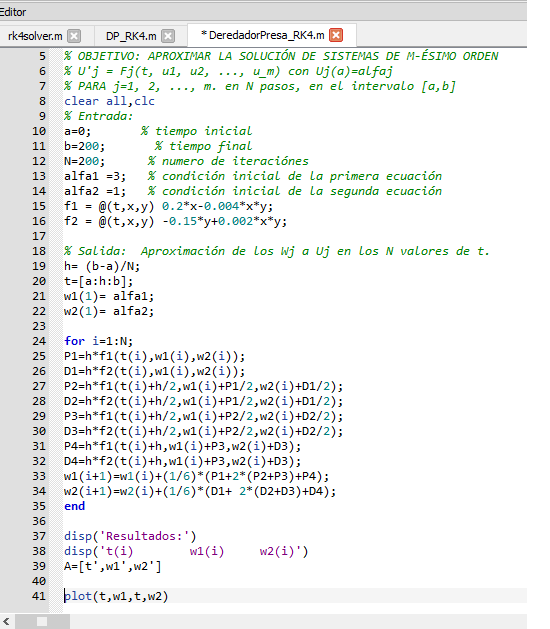
\includegraphics[scale=1]{Pic/DPcode}\\
\end{center}
\pagebreak

A continuación se muestran los resultados obtenidos mediante el método de Runge-Kutta de orden 4, en la tabla siguiente:
\begin{center}
	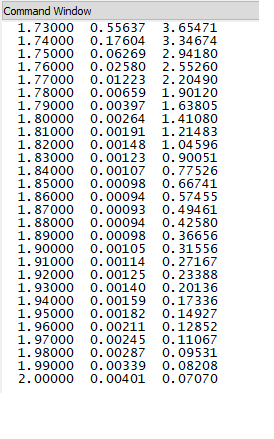
\includegraphics[scale=1]{Pic/DP00}\\
\end{center}
\pagebreak

Ahora mostramos el gráfico correspondiente, para observar el ciclo de reproducción y del problema particular. Las gráficas siguientes representan la interacción de depredadores y presas en el tiempo, reafirmando la relación previamente explicada. Por lo tanto, concluimos que el ecosistema es estable, oscilando alrededor del punto de equilibrio, es decir tiene un comportamiento cíclico:\\

Para el problema particular, tenemos,\\
 \begin{center}
 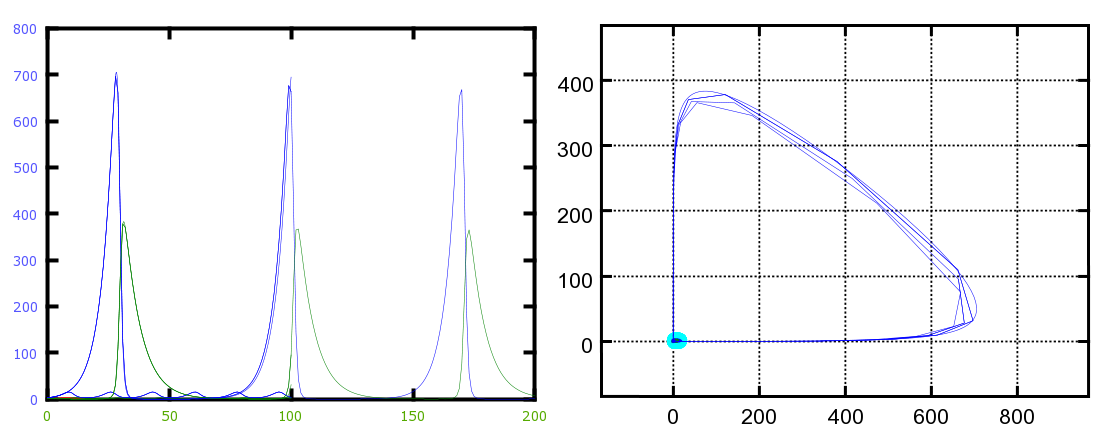
\includegraphics[scale=0.5]{Pic/DPf1}
 \end{center}
\pagebreak
Para el problema con valores iniciales a=0.4, b=0.3, c=0.37, d=0.05, tenemos,\\
\begin{center}
	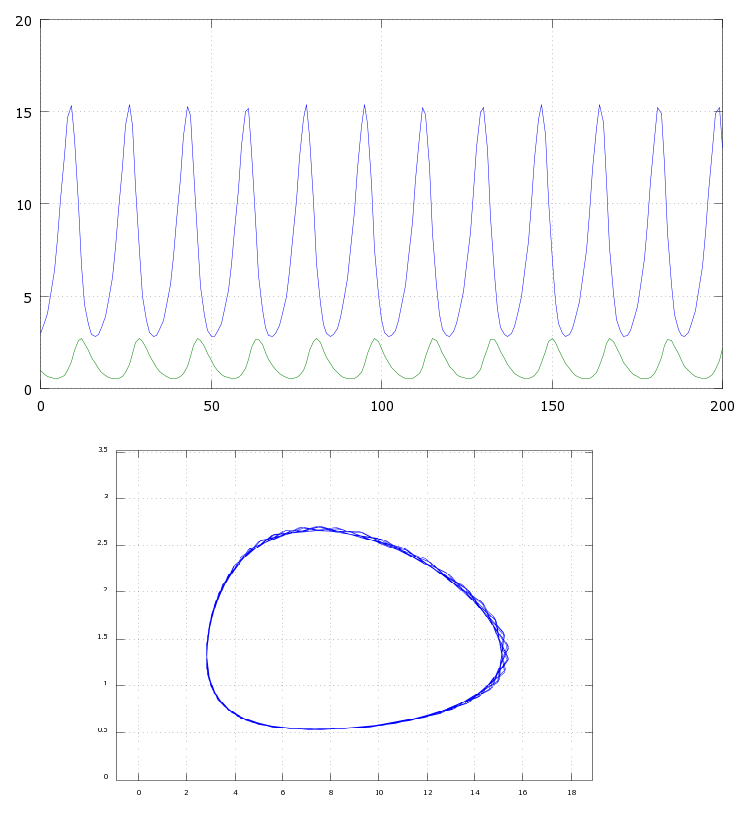
\includegraphics[scale=0.5]{Pic/DPf3}
\end{center}
\pagebreak
Para el problema con valores iniciales a=0.4, b=0.6, c=0.4, d=0.01, tenemos,\\
\begin{center}
	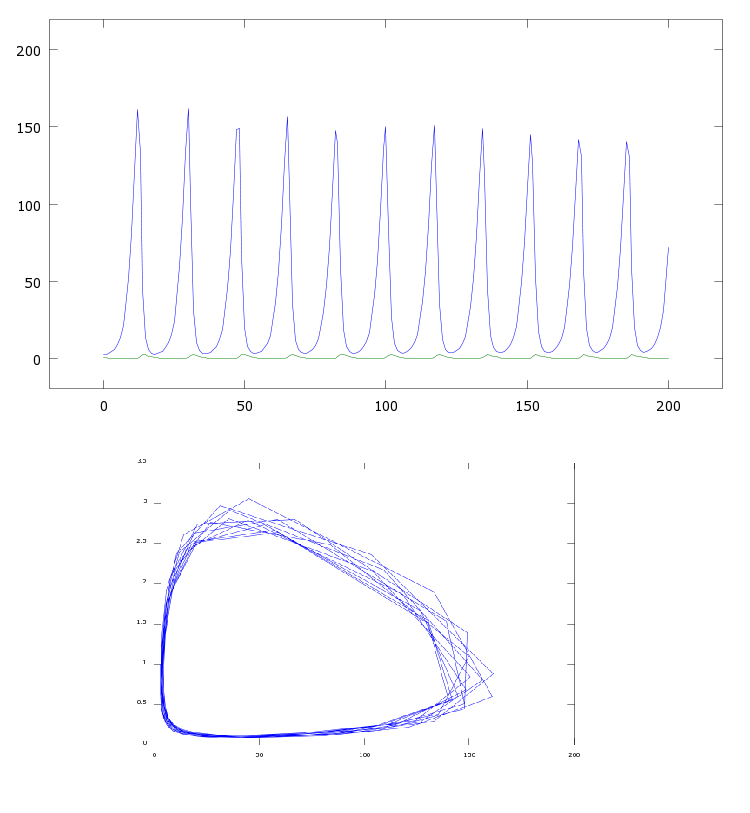
\includegraphics[scale=0.5]{Pic/DPf4}
\end{center}

\pagebreak
Para el problema con valores iniciales a=0.5, b=0.5, c=0.04, d=0.02, tenemos,\\
\begin{center}
	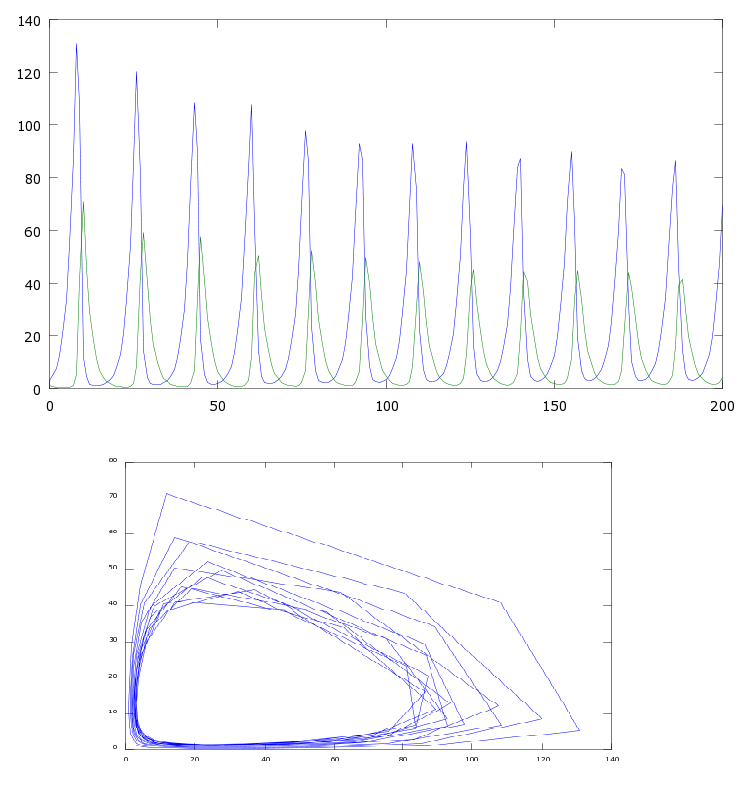
\includegraphics[scale=0.5]{Pic/DPf5}
\end{center}



\end{document}